
%(BEGIN_QUESTION)
% Copyright 2006, Tony R. Kuphaldt, released under the Creative Commons Attribution License (v 1.0)
% This means you may do almost anything with this work of mine, so long as you give me proper credit

Suppose a pressure gauge uses a diaphragm as its pressure-sensing element, like this:

$$\includegraphics[width=15.5cm]{i00172x01.eps}$$

This mechanism will work, but what if we desired to make it more sensitive?  That is, we wished to decrease its measurement span so that less pressure would drive the pointer to full-scale.  What could we alter in this mechanism to decrease the measurement span?

\underbar{file i00172}
%(END_QUESTION)





%(BEGIN_ANSWER)

Possible things to change to make this pressure-measuring mechanism more sensitive:

\begin{itemize}
\item{} Increase the area of the diaphragm
\item{} Decrease the spring rate of the diaphragm
\item{} Move the fulcrum towards the linkage, to the left, away from the scale
\end{itemize}

%(END_ANSWER)





%(BEGIN_NOTES)


%INDEX% Measurement, pressure: diaphragm

%(END_NOTES)


